\subsection{\texorpdfstring{SYSTEM OF TYPE \(E_{8}\)}{SYSTEM OF TYPE E\_8}}

\begin{enumerate}
\def\labelenumi{(\Roman{enumi})}
\tightlist
\item
  Consider the group \(\mathbf{L}_3\) (no. 4) in \(\mathbf{R}^8\) . Let \(\mathbf{R}\) be the set of \(\alpha \in \mathbf{L}_3\) such that \((\alpha |\alpha) = 2\) ; it contains the vectors
\end{enumerate}

\[
\pm \varepsilon_ {i} \pm \varepsilon_ {j} (i <   j). \frac {1}{2} \sum_ {i = 1} ^ {8} (- 1) ^ {\nu (\mathrm{i})} \varepsilon_ {i} \left(\sum_ {i = 1} ^ {8} \nu (i) \text {even}\right).
\]

Conversely, if an element \(\alpha \in L_3\) is such that \((\alpha |\alpha) = 2\) , its coordinates must be among the values \(0, \pm \frac{1}{2}, \pm 1\) ; by no. 4, either these coordinates are all integers, giving the vectors \(\pm \varepsilon_i \pm \varepsilon_j\) , or they are all equal to \(\pm \frac{1}{2}\) with an integer sum, giving the vectors

\[
\frac {1}{2} \sum_ {i = 1} ^ {8} (- 1) ^ {\nu (\mathrm{i})} \varepsilon_ {i}
\]

with \(\sum_{i=1}^{8} \nu(i)\) even.

We have seen (no. 4) that \((\alpha |\beta)\in \mathbf{Z}\) for all \(\alpha ,\beta \in \mathrm{L}_3\) . Hence, R is a reduced root system. The number of roots is \(n = \binom{8}{2}.4 + 2^7 = 240\)

\begin{enumerate}
\def\labelenumi{(\Roman{enumi})}
\setcounter{enumi}{1}
\tightlist
\item
  Let \(\rho\) be the vector \((0,1,2,3,4,5,6,23)\) of \(L_{3}\) . No element of \(R\) is orthogonal to \(\rho\) (this is clear for the \(\pm \varepsilon_{i} \pm \varepsilon_{j}\) ; if \(\frac{1}{2} \sum_{i=1}^{8} (-1)^{\nu(i)} \varepsilon_{i}\) were orthogonal to \(\rho\) , we would have \(\sum_{i=1}^{6} i(-1)^{\nu(i+1)} + 23(-1)^{\nu(8)} = 0\) , which is impossible since \(\sum_{i=1}^{6} i < 23\) ). Hence ( \(\S\) 1, no. 7, Cor. 2 of Prop. 20) the \(\alpha \in R\) such that \((\alpha | \rho) > 0\) are the positive roots relative to a certain chamber. These roots are the \(\pm \varepsilon_{i} + \varepsilon_{j}\) ( \(i < j\) ), and the
\end{enumerate}

\[
\frac {1}{2} \left(\varepsilon_ {8} + \sum_ {i = 1} ^ {7} (- 1) ^ {\nu (\mathrm{i})} \varepsilon_ {i}\right)
\]

with \(\sum_{i=1}^{7} \nu(i)\) even. We have \((\alpha|\rho) \in \mathbf{Z}\) for all \(\alpha \in \mathrm{R}\) (no. 4), and \((\alpha|\rho)\) is equal to 1 for the following roots:

\[
\alpha_ {1} = \frac {1}{2} (\varepsilon_ {1} + \varepsilon_ {8}) - \frac {1}{2} (\varepsilon_ {2} + \varepsilon_ {3} + \varepsilon_ {4} + \varepsilon_ {5} + \varepsilon_ {6} + \varepsilon_ {7}),
\]

\[
\alpha_ {2} = \varepsilon_ {1} + \varepsilon_ {2}, \alpha_ {3} = \varepsilon_ {2} - \varepsilon_ {1}, \alpha_ {4} = \varepsilon_ {3} - \varepsilon_ {2}, \alpha_ {5} = \varepsilon_ {4} - \varepsilon_ {3},
\]

\[
\alpha_ {6} = \varepsilon_ {5} - \varepsilon_ {4}, \alpha_ {7} = \varepsilon_ {6} - \varepsilon_ {5}, \alpha_ {8} = \varepsilon_ {7} - \varepsilon_ {6}.
\]

and these eight vectors form a basis of \(R^{8}\) . By § 1, no. 6, Cor. 1 of Prop. 19, \((\alpha_{1}, \alpha_{2}, \ldots, \alpha_{8})\) is a basis of R for which the positive roots are those which have been defined above. We have

\[
\left(\alpha_ {4} \mid \alpha_ {5}\right) = \left(\alpha_ {5} \mid \alpha_ {6}\right) = \left(\alpha_ {6} \mid \alpha_ {7}\right) = \left(\alpha_ {7} \mid \alpha_ {8}\right) = \left(\alpha_ {4} \mid \alpha_ {2}\right) = \left(\alpha_ {4} \mid \alpha_ {3}\right) = \left(\alpha_ {3} \mid \alpha_ {1}\right) = - 1,
\]

and \((\alpha_{i}|\alpha_{j})=0\) for all other pairs of indices. Hence, the Dynkin graph of R is of type \(E_{8}\) , and R is irreducible.

\begin{enumerate}
\def\labelenumi{(\Roman{enumi})}
\setcounter{enumi}{2}
\item
  We have \(h = \frac{n}{8} = 30\) .
\item
  Let
\end{enumerate}

\[
\tilde {\alpha} = \varepsilon_ {7} + \varepsilon_ {8} = 2 \alpha_ {1} + 3 \alpha_ {2} + 4 \alpha_ {3} + 6 \alpha_ {4} + 5 \alpha_ {5} + 4 \alpha_ {6} + 3 \alpha_ {7} + 2 \alpha_ {8},
\]

which is a root. The sum of its coordinates with respect to \((\alpha_{i})\) is 29 = h - 1, so \(\tilde{\alpha}\) is the highest root. It is orthogonal to all the \(\alpha_{i}\) except \(\alpha_{8}\) , and \((\tilde{\alpha}|\alpha_{8}) = 1\) . Hence, the completed Dynkin graph is:

\pandocbounded{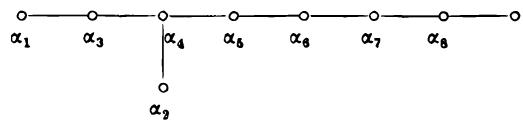
\includegraphics[keepaspectratio]{images/part002_295bff8e.jpg}}

\begin{enumerate}
\def\labelenumi{(\Alph{enumi})}
\setcounter{enumi}{21}
\tightlist
\item
  Since \((\alpha |\alpha) = 2\) for all \(\alpha \in \mathbb{R}\) , we have \(R^{\prime} = R\) .
\end{enumerate}

For \(\Phi_{\mathrm{R}}\) , the squared length of the roots is \(\frac{1}{30}\) ( \(\S 1\) , no. 12). Hence, \(\Phi_{\mathrm{R}}(x,y) = (x|y)/60\) and \(\gamma(\mathrm{R}) = 900\) ( \(\S 1\) , no. 12, formula (20)).

\begin{enumerate}
\def\labelenumi{(\Roman{enumi})}
\setcounter{enumi}{5}
\tightlist
\item
  Calculating the fundamental weights gives
\end{enumerate}

\[
\begin{array}{l} \omega_ {1} = 2 \varepsilon_ {8} = 4 \alpha_ {1} + 5 \alpha_ {2} + 7 \alpha_ {3} + 10 \alpha_ {4} + 8 \alpha_ {5} + 6 \alpha_ {6} + 4 \alpha_ {7} + 2 \alpha_ {8} \\ \omega_ {2} = \frac {1}{2} (\varepsilon_ {1} + \varepsilon_ {2} + \varepsilon_ {3} + \varepsilon_ {4} + \varepsilon_ {5} + \varepsilon_ {6} + \varepsilon_ {7} + 5 \varepsilon_ {8}) \\ \qquad = 5 \alpha_ {1} + 8 \alpha_ {2} + 10 \alpha_ {3} + 15 \alpha_ {4} + 12 \alpha_ {5} + 9 \alpha_ {6} + 6 \alpha_ {7} + 3 \alpha_ {8} \\ \omega_ {3} = \frac {1}{2} (- \varepsilon_ {1} + \varepsilon_ {2} + \varepsilon_ {3} + \varepsilon_ {4} + \varepsilon_ {5} + \varepsilon_ {6} + \varepsilon_ {7} + 7 \varepsilon_ {8}) \\ \qquad = 7 \alpha_ {1} + 10 \alpha_ {2} + 14 \alpha_ {3} + 20 \alpha_ {4} + 16 \alpha_ {5} + 12 \alpha_ {6} + 8 \alpha_ {7} + 4 \alpha_ {8} \\ \omega_ {4} = \varepsilon_ {3} + \varepsilon_ {4} + \varepsilon_ {5} + \varepsilon_ {6} + \varepsilon_ {7} + 5 \varepsilon_ {8} \\ \qquad = 10 \alpha_ {1} + 15 \alpha_ {2} + 20 \alpha_ {3} + 30 \alpha_ {4} + 24 \alpha_ {5} + 18 \alpha_ {6} + 12 \alpha_ {7} + 6 \alpha_ {8} \\ \omega_ {5} = \varepsilon_ {4} + \varepsilon_ {5} + \varepsilon_ {6} + \varepsilon_ {7} + 4 \varepsilon_ {8} \\ \qquad = 8 \alpha_ {1} + 12 \alpha_ {2} + 16 \alpha_ {3} + 24 \alpha_ {4} + 20 \alpha_ {5} + 15 \alpha_ {6} + 10 \alpha_ {7} + 5 \alpha_ {8} \\ \omega_ {6} = \varepsilon_ {5} + \varepsilon_ {6} + \varepsilon_ {7} + 3 \varepsilon_ {8} \\ \qquad = 6 \alpha_ {1} + 9 \alpha_ {2} + 12 \alpha_ {3} + 18 \alpha_ {4} + 15 \alpha_ {5} + 12 \alpha_ {6} + 8 \alpha_ {7} + 4 \alpha_ {8} \\ \omega_ {7} = \varepsilon_ {6} + \varepsilon_ {7} + 2 \varepsilon_ {8} \\ \qquad = 4 \alpha_ {1} + 6 \alpha_ {2} + 8 \alpha_ {3} + 2 \alpha_ {4} + 10 \alpha_ {5} + 8 \alpha_ {6} + 6 \alpha_ {7} + 3 \alpha_ {8} \\ \omega_ {8} = \varepsilon_ {7} + \varepsilon_ {8} \\ \qquad = 5 \alpha_ {1} + 8 \alpha_ {2} + 10 \alpha_ {3} + 15 \alpha_ {4} + 12 \alpha_ {5} + 9 \alpha_ {6} + 6 \alpha_ {7} + 3 \alpha_ {8} = \tilde {\alpha}. \end{array}
\]

\begin{enumerate}
\def\labelenumi{(\Roman{enumi})}
\setcounter{enumi}{6}
\tightlist
\item
  Half the sum of the positive roots is the sum of the fundamental weights (§ 1, no. 10, Prop. 29); this gives
\end{enumerate}

\[
\begin{array}{r l} \rho & = \varepsilon_ {2} + 2 \varepsilon_ {3} + 3 \varepsilon_ {4} + 4 \varepsilon_ {5} + 5 \varepsilon_ {6} + 6 \varepsilon_ {7} + 23 \varepsilon_ {8} \\ & = 46 \alpha_ {1} + 68 \alpha_ {2} + 91 \alpha_ {3} + 135 \alpha_ {4} + 110 \alpha_ {5} + 84 \alpha_ {6} + 57 \alpha_ {7} + 29 \alpha_ {8}. \end{array}
\]

\begin{enumerate}
\def\labelenumi{(\Roman{enumi})}
\setcounter{enumi}{7}
\item
  The group \(Q(R)\) is generated by the \(\varepsilon_{i} \pm \varepsilon_{j}\) and \(\frac{1}{2} \sum_{i=1}^{8} \varepsilon_{i}\) , and is equal to \(L_{3}\) (no. 4). Hence \(P(R)\) , which is associated to \(Q(R^{\prime}) = Q(R) = L_{3}\) , is \(L_{3}\) (no. 4). The connection index is 1.
\item
  The family of exponents has 8 terms, and since h = 30, the integers 1, 7, 11, 13, 17, 19, 23, 29, coprime to 30, must feature in this family; consequently, these are the exponents of W(R).
\item
  From (IX) and Chap. V, § 6, no. 2, Cor. 1 of Prop. 3, it follows that the order of W(R) is
\end{enumerate}

\[
2. 8. 12. 14. 18. 20. 24. 30 = 2 ^ {14}. 3 ^ {5}. 5 ^ {2}. 7.
\]

\begin{enumerate}
\def\labelenumi{(\Roman{enumi})}
\setcounter{enumi}{10}
\tightlist
\item
  The only automorphism of the Dynkin graph is the identity since the three chains issuing from the ramification point have distinct lengths. Hence, \(A(R) = W(R)\) and \(w_{0} = -1\) .
\end{enumerate}

